This section is new in this report. It asks whether the improvements are larger than what chance and the choice of test sessions could produce (script \texttt{fr\_bootstrap.py}). The test windows of one session overlap and share the regime of that session, so the unit of independent evidence is the session, not the window. We therefore resample whole test sessions with replacement (2000 replicates, paired for the two models) and read the 95\% percentile interval of the change.

\begin{table}[H]
\centering
\caption{RTT on the test sessions, averaged over 0.2--3\,s, for the three-seed ensembles S2S-E and DS2S-E. Changes of DS2S-E against S2S-E with 95\% session-bootstrap intervals. Bold: the interval excludes zero. MAE uses the median of DS2S-E, RMSE the means. IS and PICP refer to the calibrated 95\% interval.}
\label{tab:boot}
\resizebox{\linewidth}{!}{%
\begin{tabular}{l rrr rrr rrr cc}
\toprule
 & \multicolumn{3}{c}{Interval score (ms)} & \multicolumn{3}{c}{MAE (ms)} & \multicolumn{3}{c}{RMSE (ms)} & \multicolumn{2}{c}{PICP} \\
\cmidrule(lr){2-4}\cmidrule(lr){5-7}\cmidrule(lr){8-10}\cmidrule(lr){11-12}
Link & S2S-E & DS2S-E & $\Delta$\% [95\% CI] & S2S-E & DS2S-E & $\Delta$\% [95\% CI] & S2S-E & DS2S-E & $\Delta$\% [95\% CI] & S2S-E & DS2S-E \\
\midrule
\tabinput{data/tab_main_boot.tex}
\bottomrule
\end{tabular}}
\end{table}

\begin{figure}[H]
  \centering
  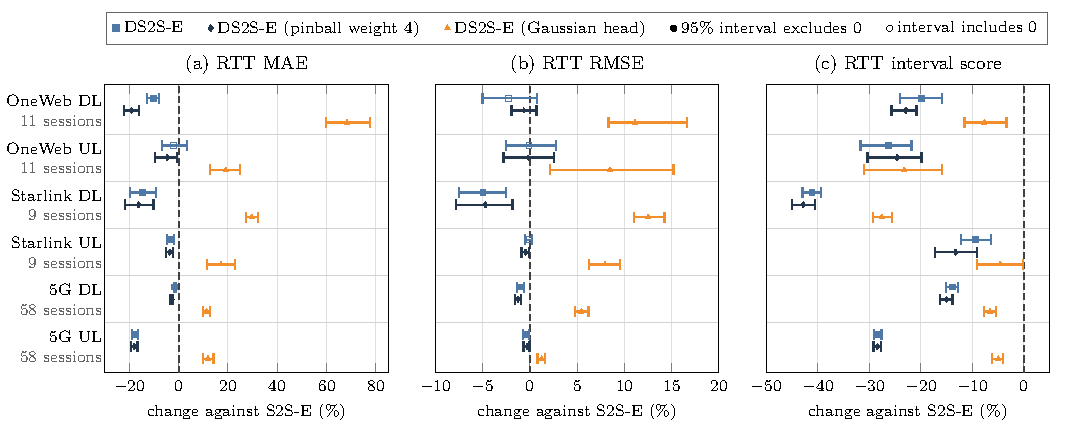
\includegraphics[width=\linewidth]{figs_pdf/fr_bootstrap.pdf}
  \caption{Session-level bootstrap of the RTT change of DS2S-E against S2S-E (2000 replicates). Marker: bootstrap median. Bar: 95\% percentile interval. Filled: the interval excludes zero. Negative values favor DS2S-E.}
  \label{fig:bootstrap}
\end{figure}

\paragraph{Results.} Table~\ref{tab:boot} and Fig.~\ref{fig:bootstrap} give the changes with their intervals. The interval score improves significantly on all six links, and DS2S-E has the lower interval score in each of the \BSnSessTot{} test sessions. The MAE improves significantly on five links and is inconclusive on OneWeb UL. The RMSE improves significantly on three links (Starlink DL, 5G DL, 5G UL) and is inconclusive on the other three. No change is significantly worse.

\paragraph{Why sessions and not windows.} A bootstrap over windows treats the \BSnWinTot{} overlapping test windows as independent. It gives intervals \BSWidRatioLo{} to \BSWidRatioHi{} times narrower than the session bootstrap and would call two inconclusive changes significant, the RMSE on OneWeb DL and the MAE on OneWeb UL. With 9 to 11 test sessions per satellite link, the evidence is closer to 11 independent pieces than to 27{,}000.

\paragraph{Robustness.} Leaving out any one test session moves the interval-score change by at most \BSLooMax{} points. With intervals from the empirical quantiles of the test residuals, the protocol of the previous report, DS2S-E and S2S-E are within \IsProtoMaxAbs\% of each other on every link, because both intervals then have a constant width. The gain is visible only with intervals calibrated on held-out sessions. On Starlink DL the comparison holds on the measured targets alone, without the parser-interpolated ones (MAE \RealMAEFRSLDL{} against \RealMAEPrevSLDL\,ms).

\paragraph{Caveats.} The intervals are conditional on the trained ensembles and on the calibration offsets learned on the calibration sessions, which are held fixed in each replicate. They do not include seed variability. Sessions come from one campaign per link, so the intervals do not cover other seasons, terminals, or years.
